\documentclass[border=4pt]{standalone}
\usepackage{tikz}
\usetikzlibrary{decorations.pathmorphing}
\begin{document}
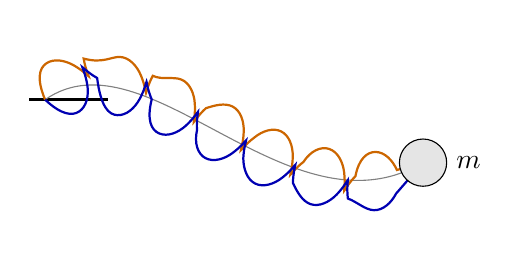
\begin{tikzpicture}
  \draw[very thick] (-.2,1.5) -- (.8,1.5);
  \draw[gray] (0,1.5) .. controls (1.3,2.4) and (3.1,-.3) .. (4.8,.7);
  \draw[orange!80!black,thick,decorate,
    decoration={coil,segment length=7mm,amplitude=2.2mm,aspect=.45,raise=1.5mm}]
    (0,1.5) .. controls (1.3,2.4) and (3.1,-.3) .. (4.8,.7);
  \draw[blue!70!black,thick,decorate,
    decoration={coil,segment length=7mm,amplitude=2.2mm,aspect=.45,mirror,raise=1.5mm}]
    (0,1.5) .. controls (1.3,2.4) and (3.1,-.3) .. (4.8,.7);
  \draw[fill=gray!20] (4.8,.7) circle (3mm);
  \node[right] at (5.1,.7) {$m$};
\end{tikzpicture}
\end{document}
